\documentclass[12pt]{beamer}
\usetheme{Madrid}
\usepackage[utf8]{inputenc}
\usepackage[english]{babel}
\usepackage{amsmath}
\usepackage{amsfonts}
\usepackage{amssymb}
\usepackage{multicol}
\usepackage{graphicx}
\graphicspath{ {./images/} }

\author[Edgar, Shah, Ronald]{Edgar Luque \and Shah Sawar \and Ronald Intriago}
\title{Gymodo}
\subtitle{The best app for your gym} 


\definecolor{gymodo_orange}{rgb}{1, 0.556, 0.235}

\definecolor{UBCblue}{rgb}{0.04706, 0.13725, 0.26667}
\usecolortheme[named=UBCblue]{structure}

%\setbeamercovered{transparent} 
%\setbeamertemplate{navigation symbols}{} 
\logo{
\includegraphics[height=1cm]{gymodo_logo}} 
\institute[2WIAM]{
Multiplatform App Development Project\\
2WIAM \\
Escola del Treball de Barcelona
} 
\date{\today} 

\begin{document}

\begin{frame}
\titlepage
\end{frame}

\begin{frame}
\frametitle{Índice}
\tableofcontents
\end{frame}

\section{Abstract}
\begin{frame}{Abstract}

\textbf{\color{gymodo_orange} Gymodo} is an android whose main objective is to solve the problems that arose due to the global pandemic and these modern times.

\begin{itemize}
\item Reserve hour at a gym
\item Create workouts
\item Create diets with the ability to scan food
\item View related news
\item Create posts with comments, a small social network
\end{itemize}

\end{frame}

\section{View of the app}
\begin{frame}{View of the app}

\begin{center}
\includegraphics[width=0.23\textwidth]{gymodo_home}
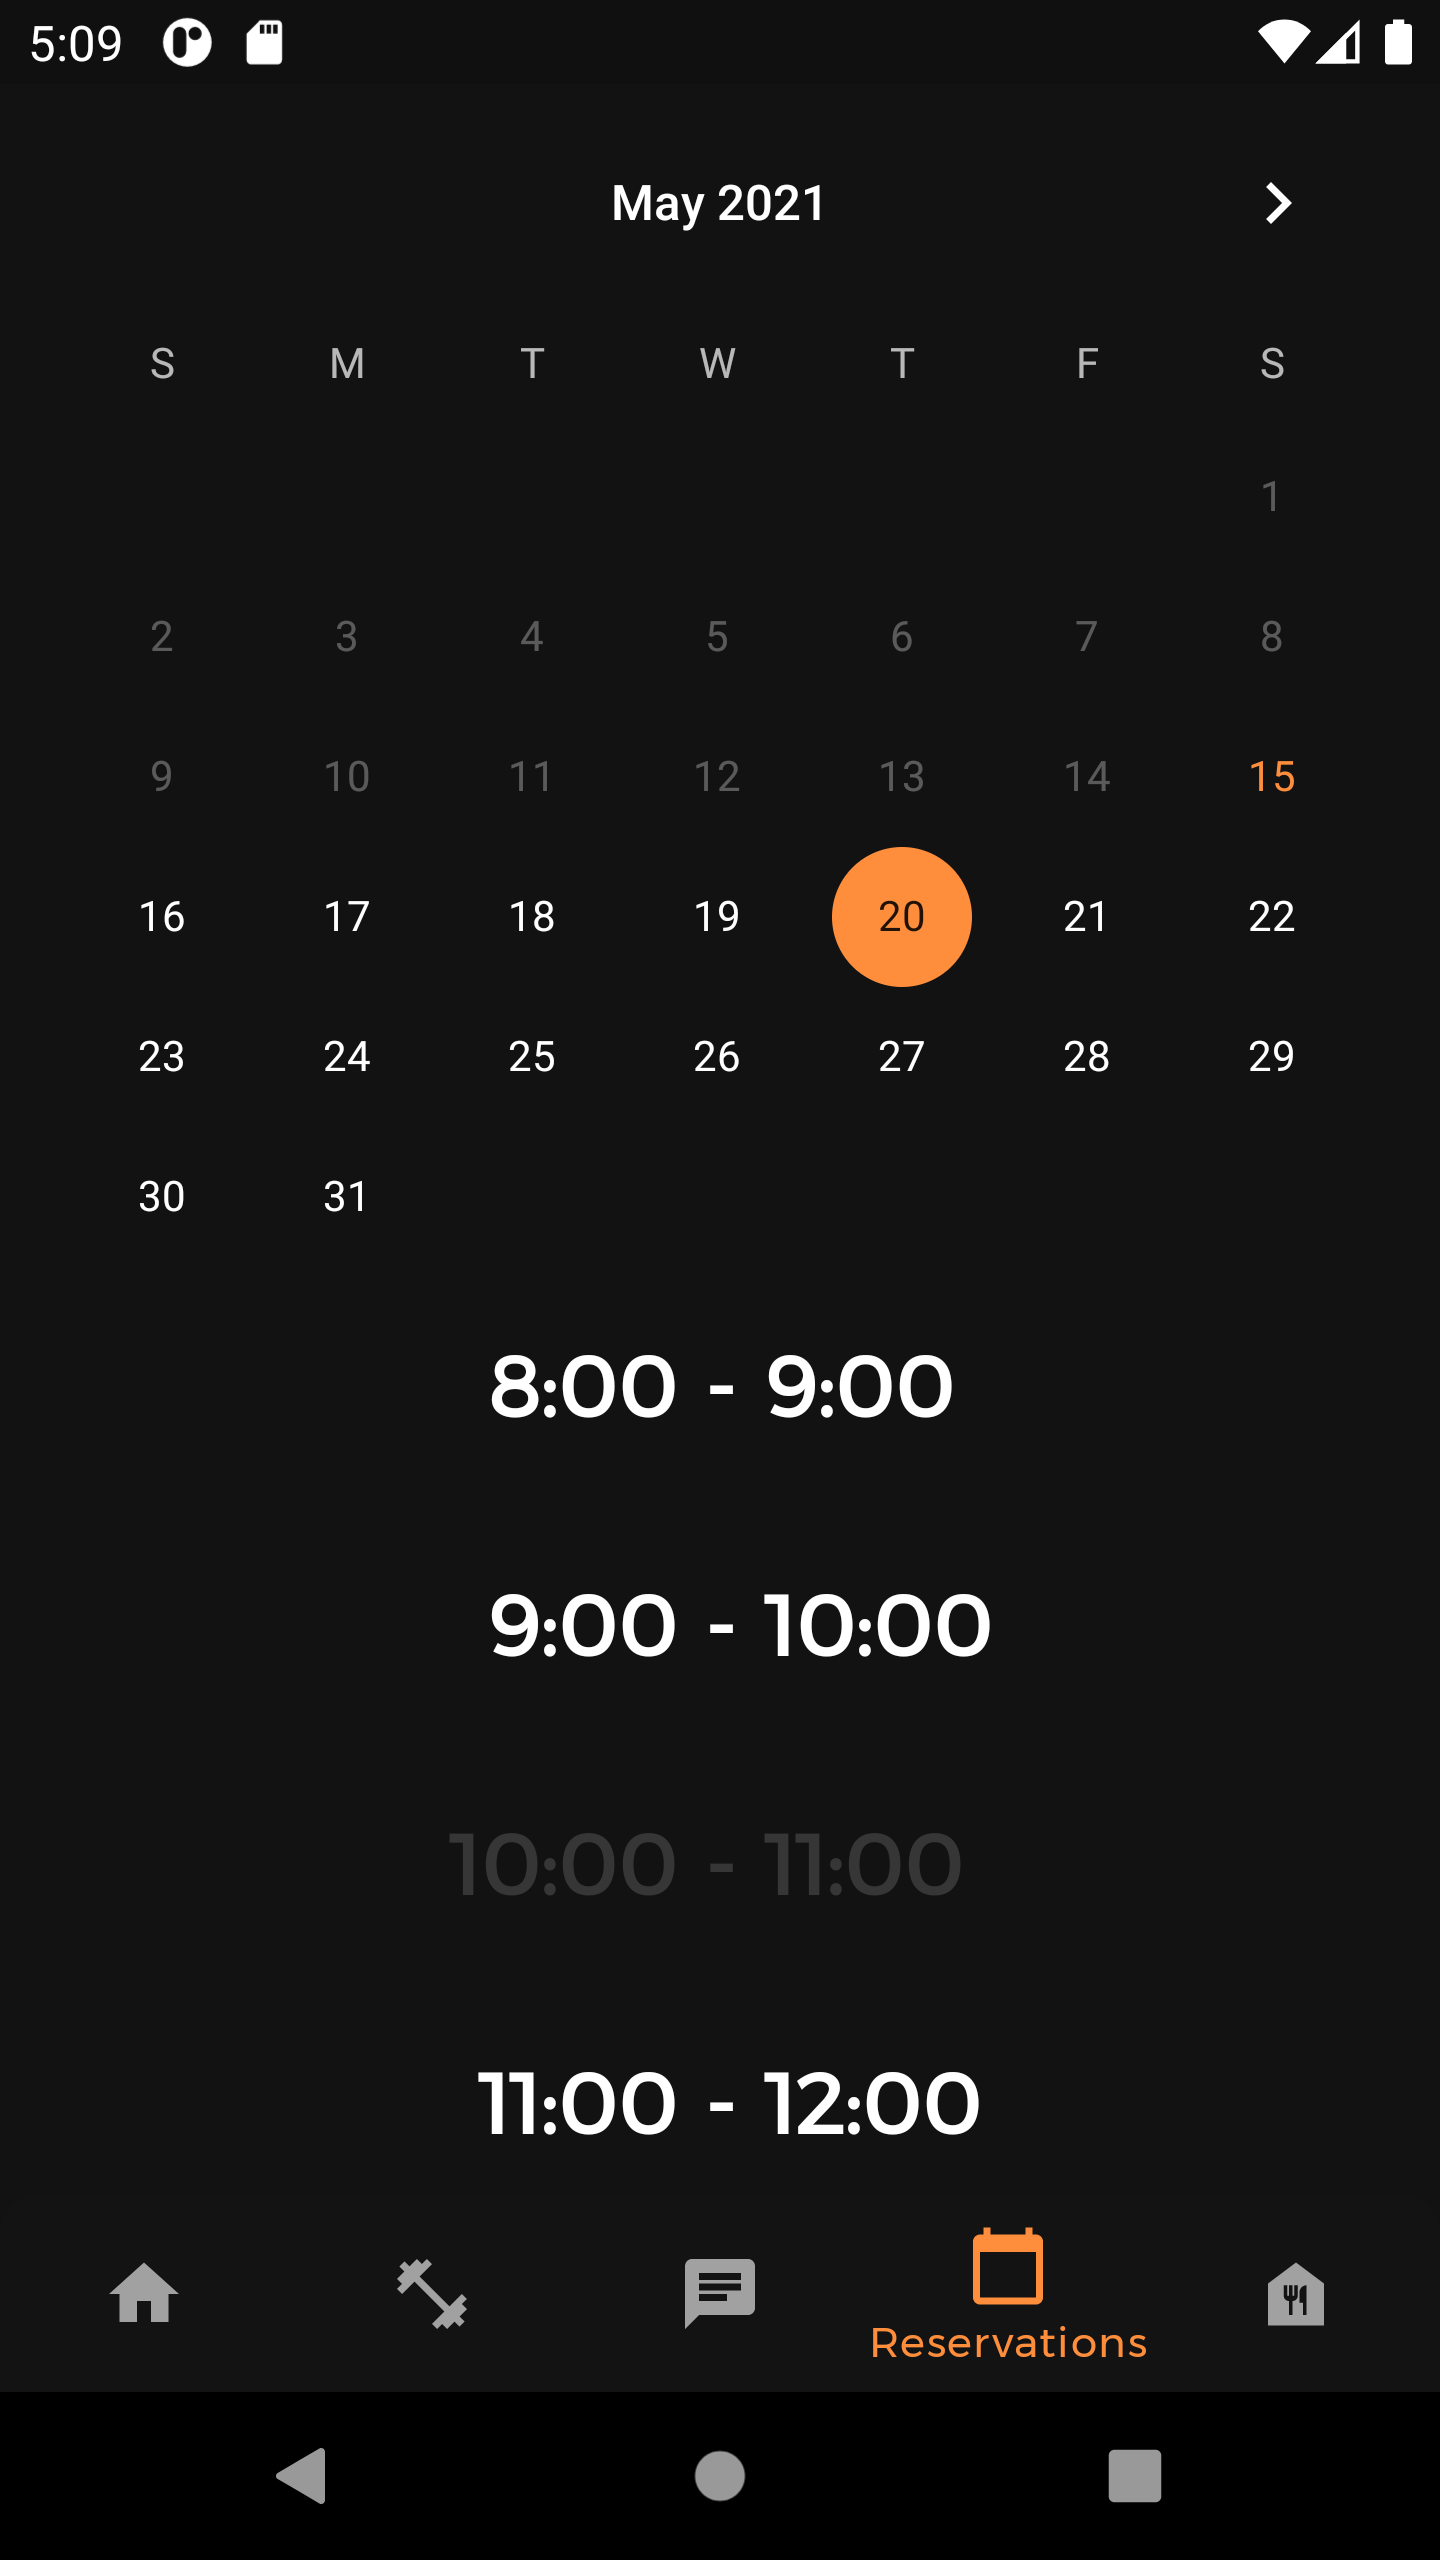
\includegraphics[width=0.23\textwidth]{gymodo_create_reservation}
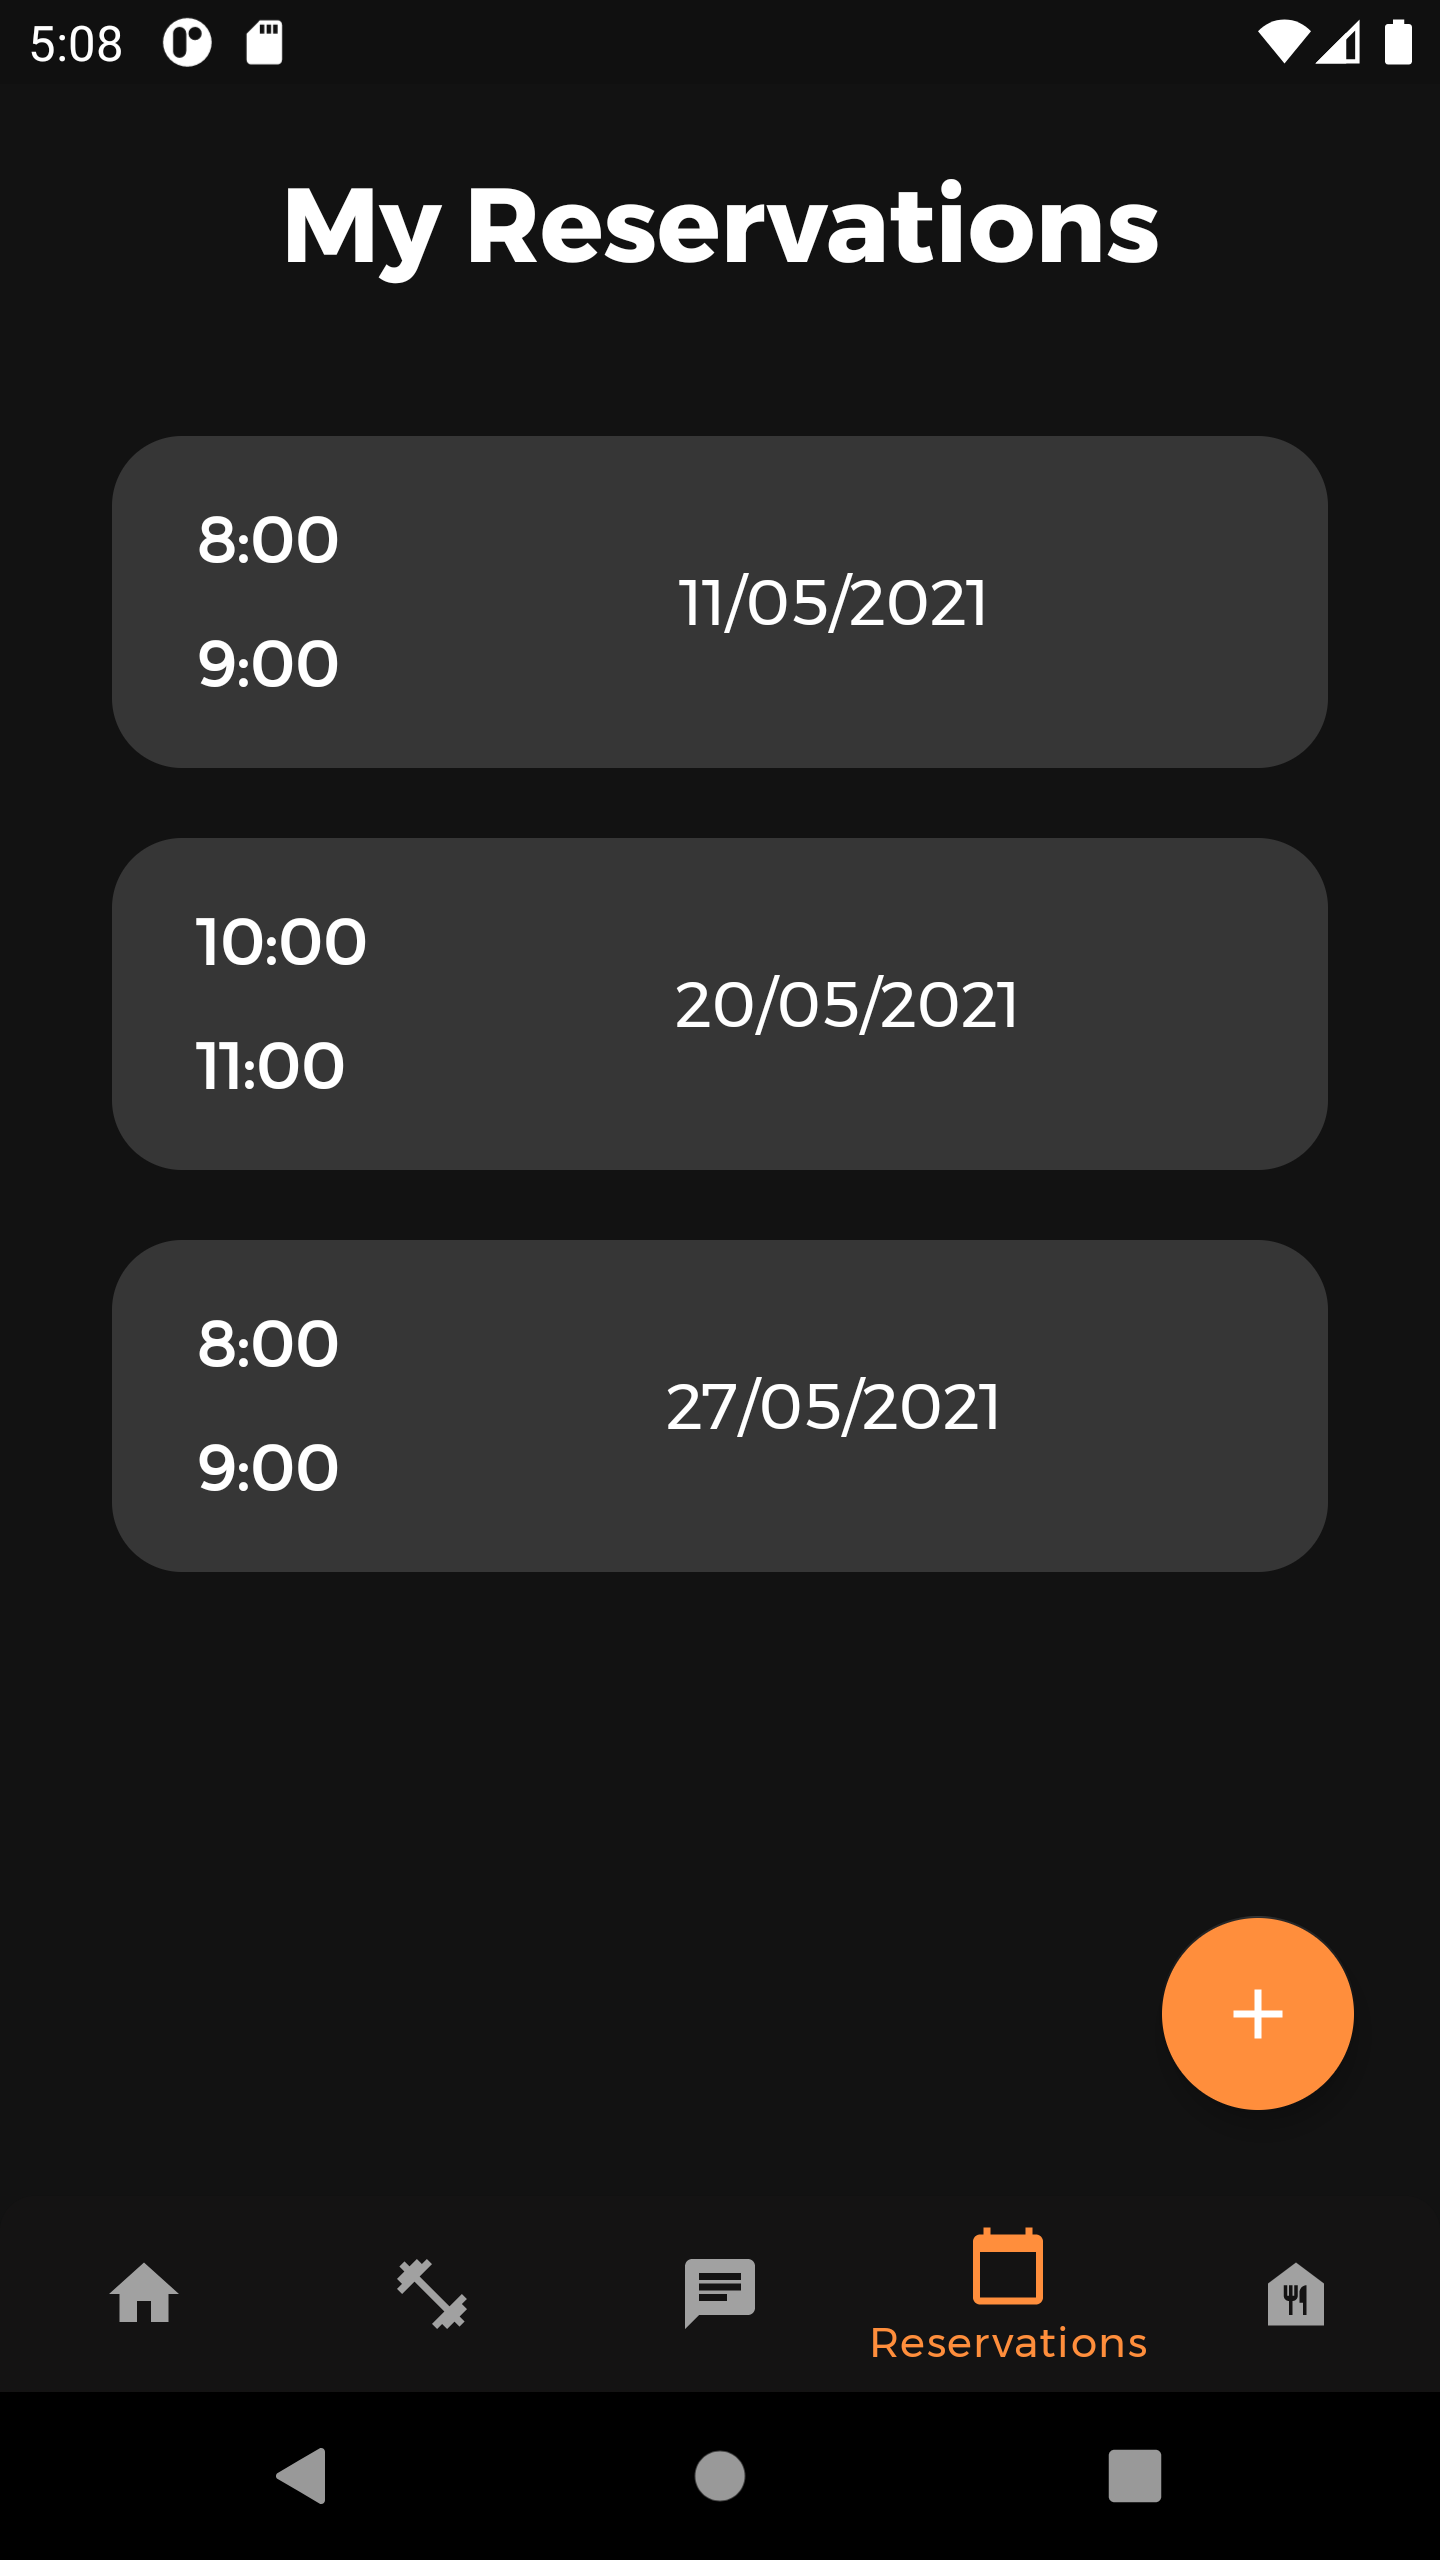
\includegraphics[width=0.23\textwidth]{gymodo_your_reservations}
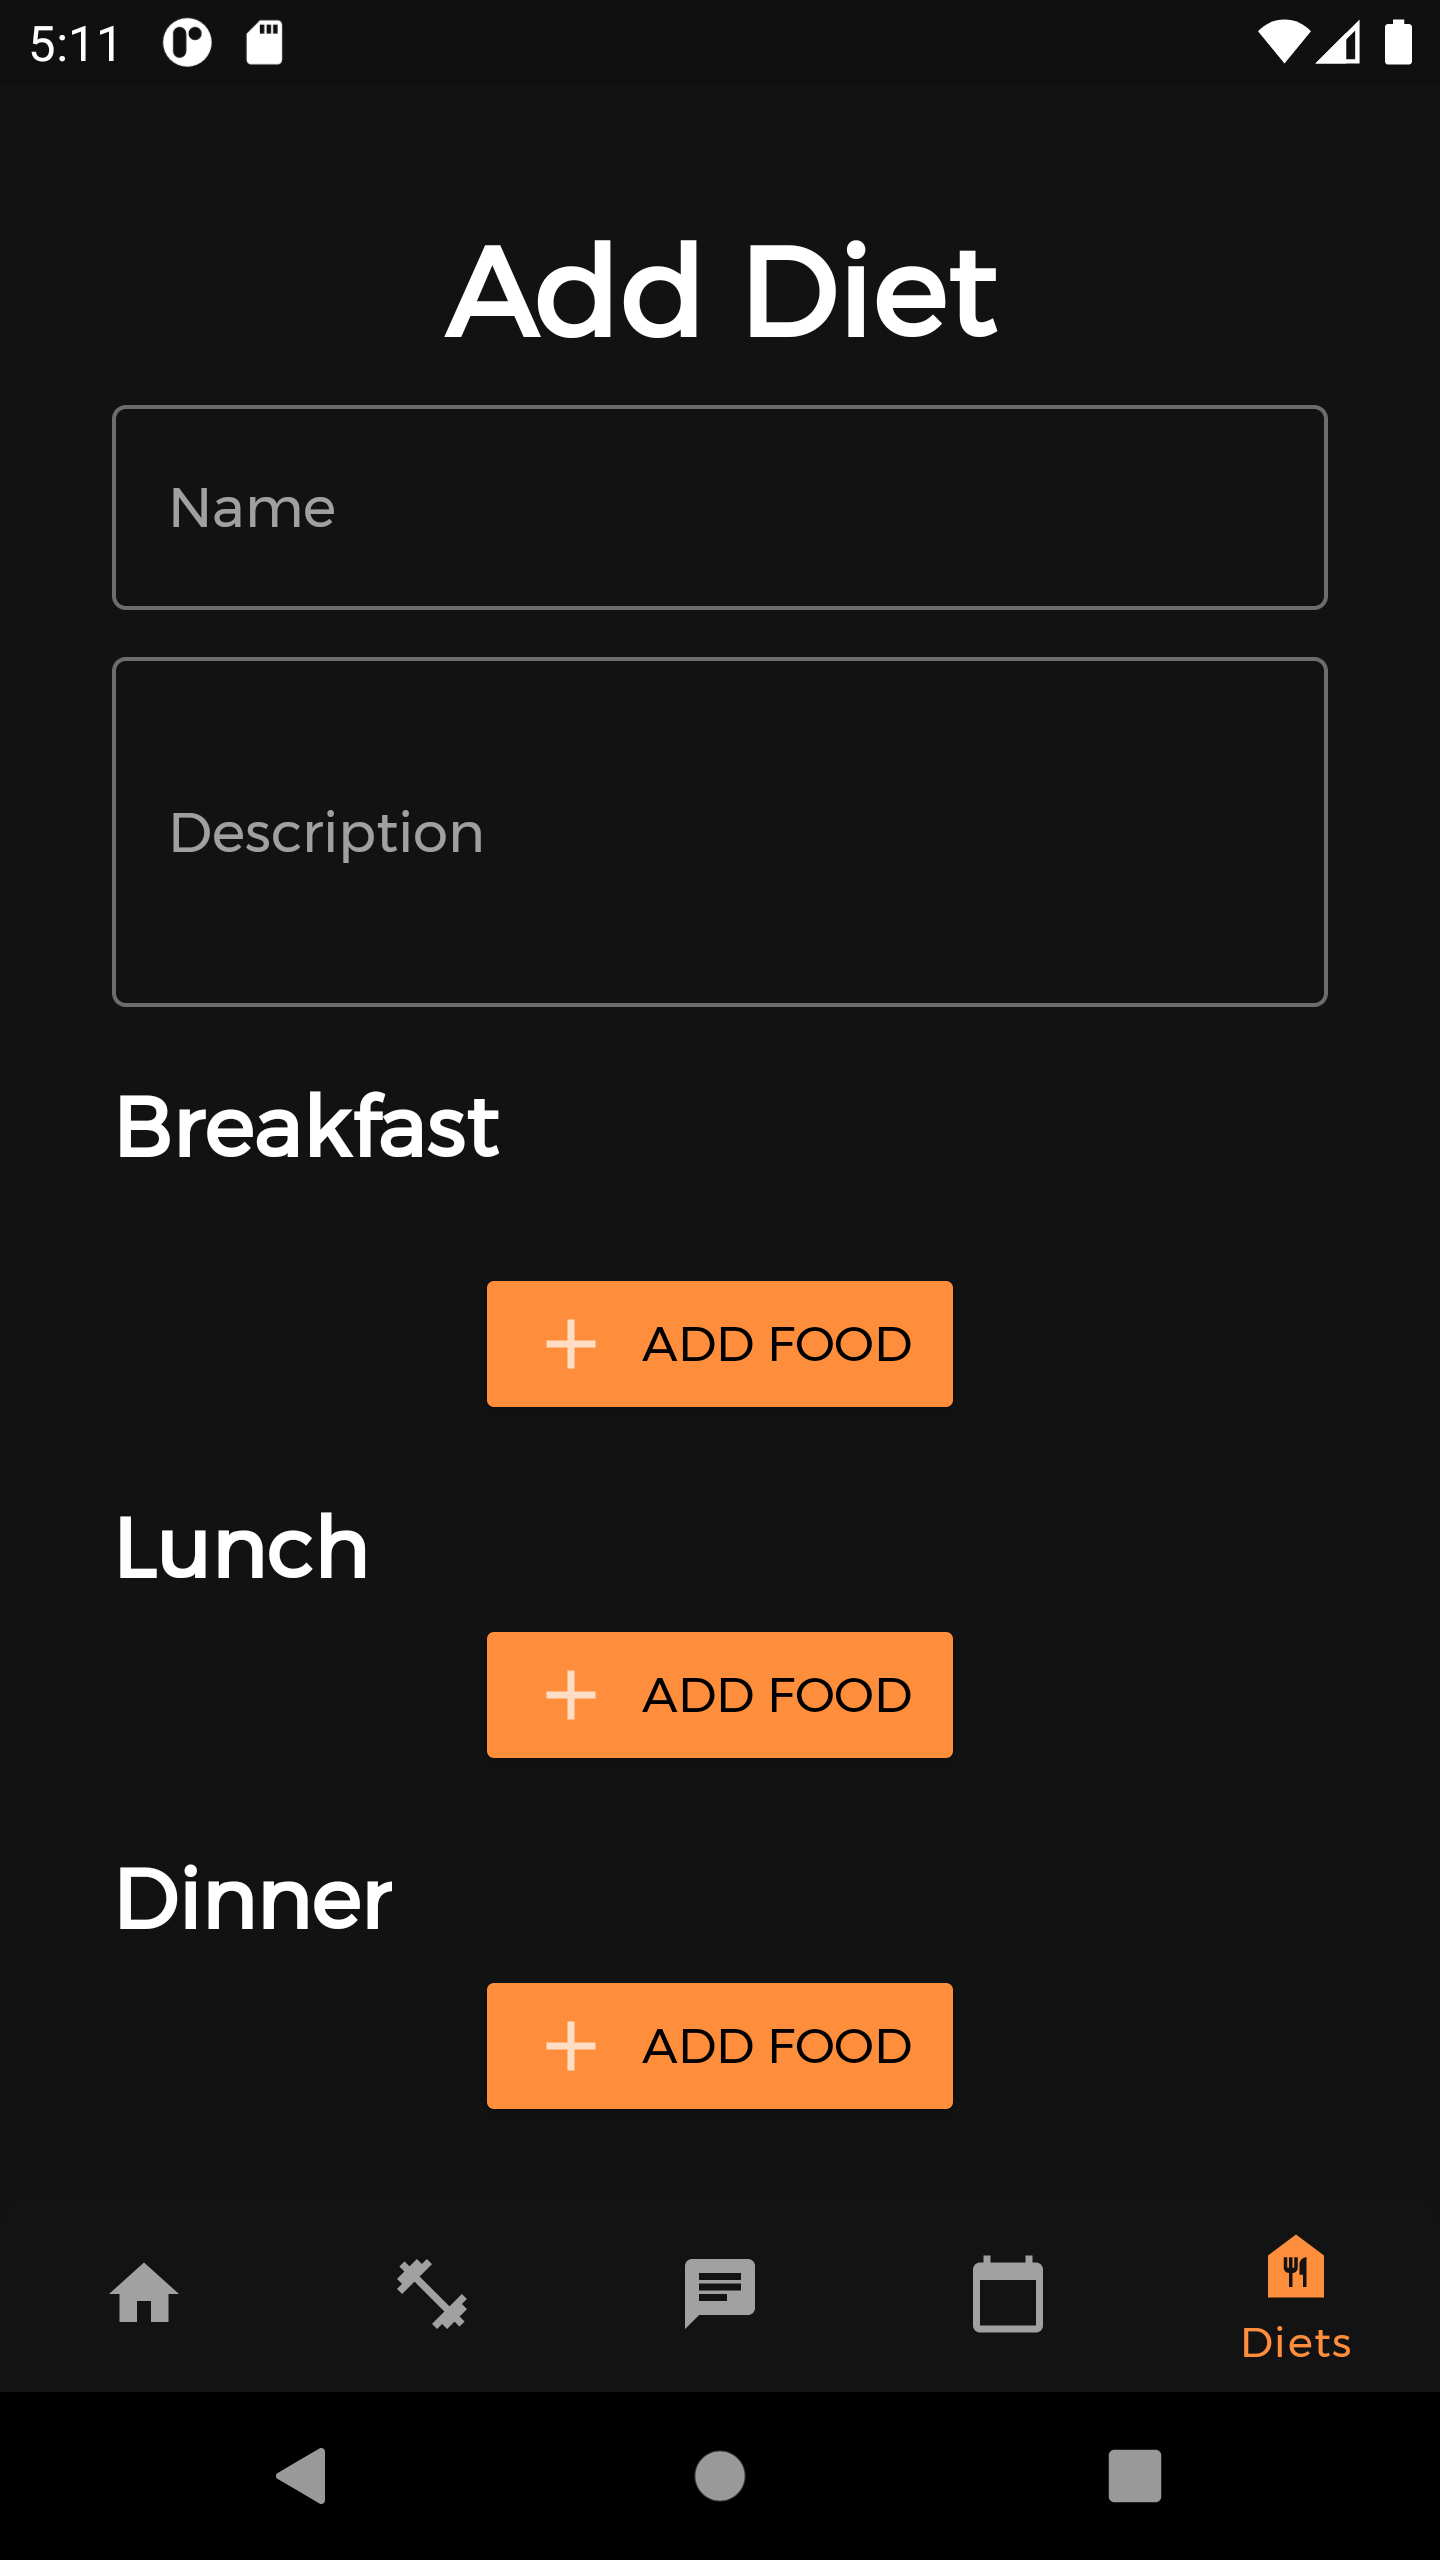
\includegraphics[width=0.23\textwidth]{gymodo_add_diet}
\end{center}

\end{frame}

\section{Technology Stack}
\begin{frame}{Technology Stack}

\begin{center}


\includegraphics[width=0.2\textwidth]{asana}

\includegraphics[width=0.2\textwidth]{mlkit}

\includegraphics[width=0.2\textwidth]{androidstudio}


\includegraphics[width=0.2\textwidth]{firebase}

\includegraphics[width=0.2\textwidth]{toggl}

\includegraphics[width=0.2\textwidth]{git}
{\LARGE \LaTeX}
\end{center}
\end{frame}

\section{Diseño}
\begin{frame}{Design}

\begin{center}
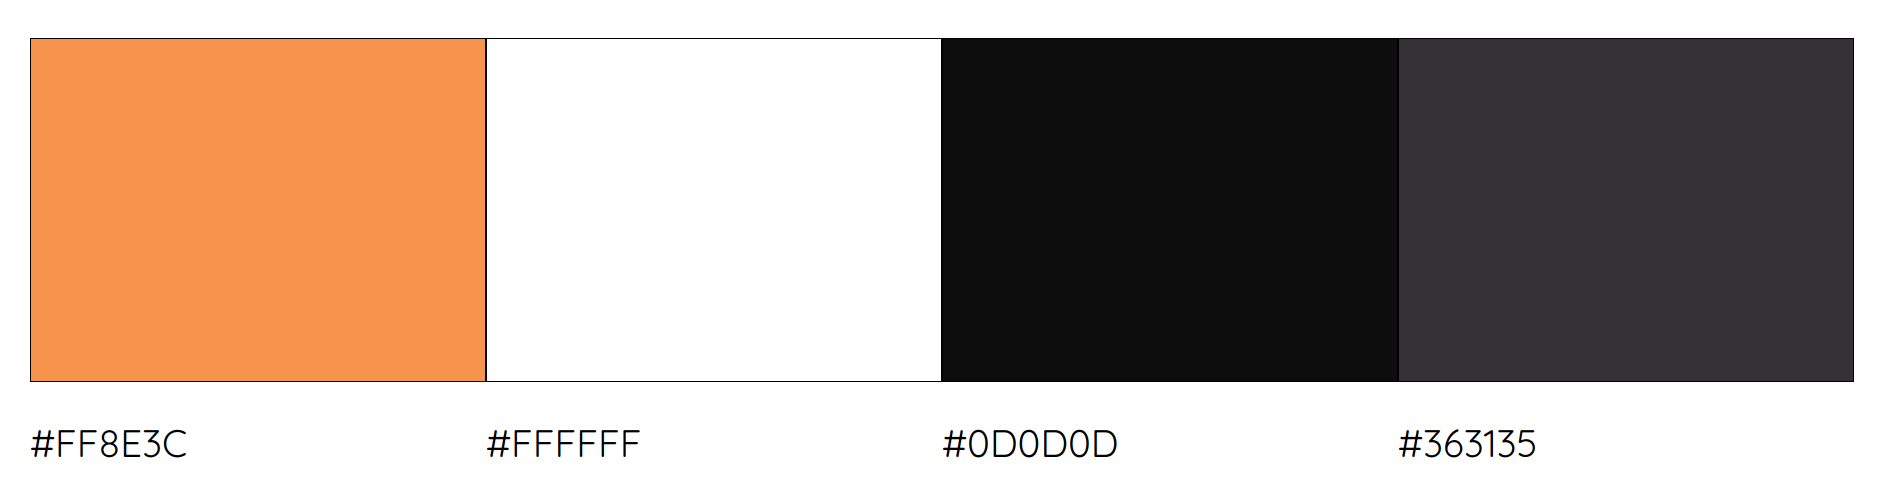
\includegraphics[width=\textwidth]{color_palette}

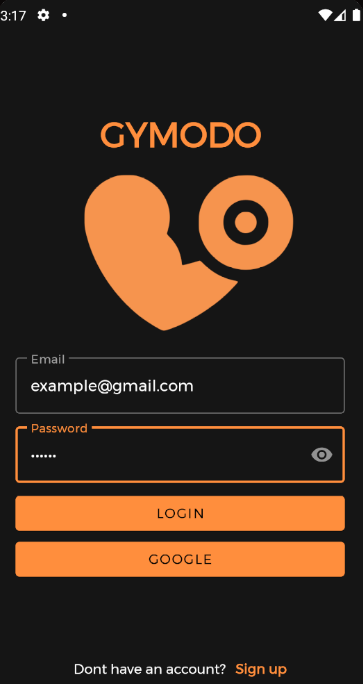
\includegraphics[height=0.45\textheight]{loginconcredenciales}

\includegraphics[width=0.4\textwidth]{gymodo_logo}
\end{center}


\end{frame}

\section{Development phases}
\begin{frame}{Development phases}

\begin{enumerate}
\item Diagrams:

\begin{itemize}
\item Class diagram.
\item Entity-Relationship diagram.
\item Use case.
\end{itemize}

\item Design mockup.

\item Configure firebase.

\item Create classes from the diagrams.

\item Create the design layouts.

\item Implement the view functionality.

\item Create the documentation.

\end{enumerate}
\end{frame}

\section{Statistics}
\begin{frame}{Statistics}

\only<1> {
\framesubtitle{Toggl}
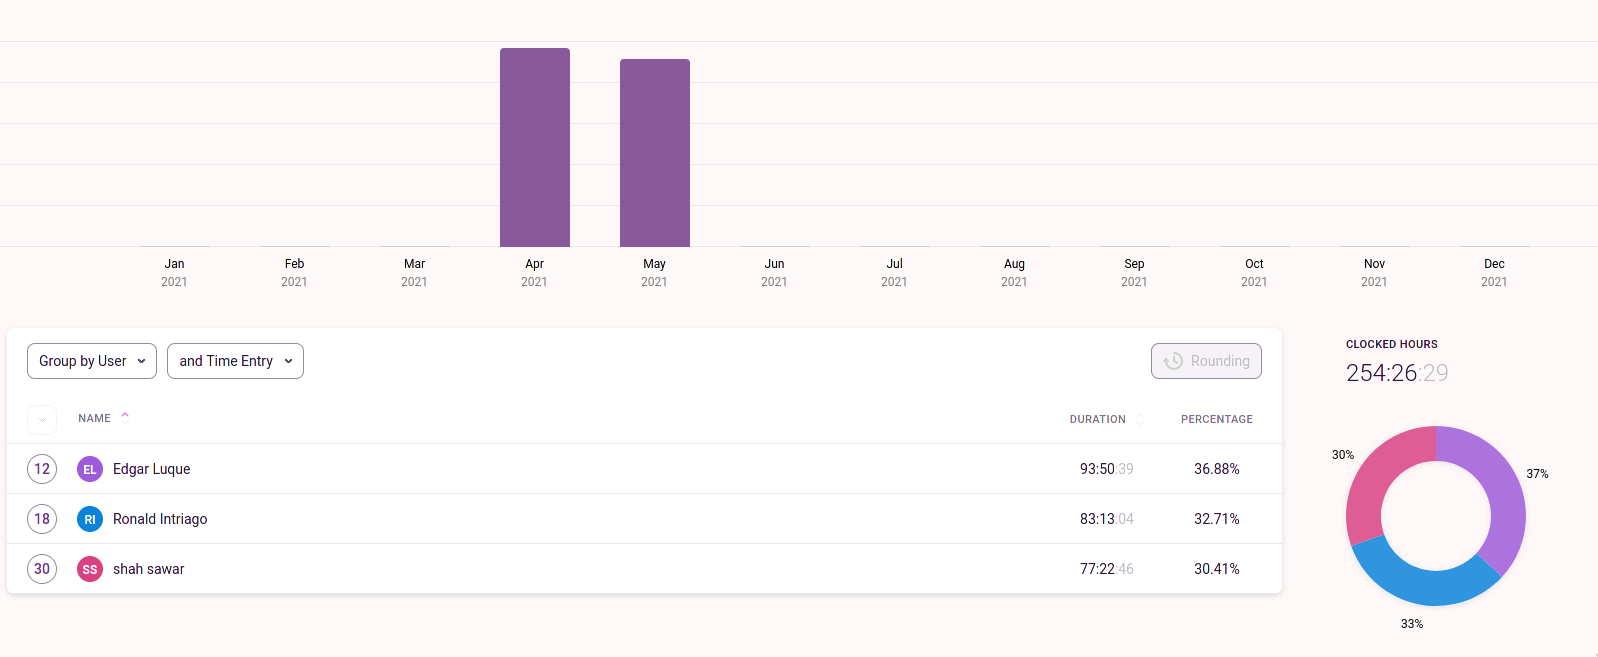
\includegraphics[width=\textwidth]{toggl-stats}
}

\only<2> {
\framesubtitle{Github}

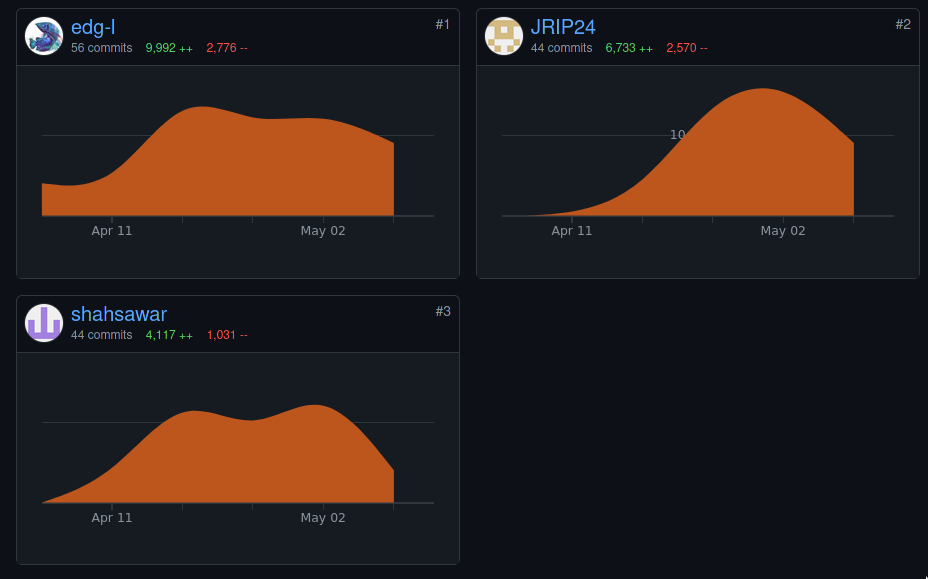
\includegraphics[width=0.92\textwidth]{git-contributors}
}

\end{frame}


\section{Conclusion}
\begin{frame}{Conclusion}

Que hemos aprendido:

\begin{itemize}
\item Git
\item Android
\item Firebase
\item \LaTeX
\item Teamwork
\end{itemize}


\end{frame}

\section{Questions}
\begin{frame}{Questions}

\begin{center}

\includegraphics[width=0.8\textwidth]{gymodo_logo}
\end{center}


\end{frame}

\end{document}